\documentclass[../../dissertation.tex]{subfiles}
\begin{document}
\chapter{Domestic Politics, Territorial Claims, and Economic Interdependence}

% \footnote{This article has not been submitted for publication.}

% Introduction

Does economic interdependence promote the peaceful settlement of contentious issue claims between states? An extensive body of research argues that states engaged in high levels of bilateral economic activity are less likely to fight militarized disputes. Because military conflict reduces economic activity between states, the prospect of fighting threatens the interests of powerful actors dependent on trade. As a result, these actors have an incentive to pressure leaders to avoid military conflict. 

% Theory

Despite the extensive body of literature on trade and military disputes, few studies consider the possibility that interdependence facilitates the resolution of the issues over which states compete \citep[exceptions include][]{lee2012, schultz2015}. Even in the absence of militarized conflict, issue claims can reduce the extent of economic activity between states by influencing individuals’ expectations about the future likelihood of military and diplomatic conflict and by creating uncertainty about who possesses jurisdiction over the issue claim. This hinders bilateral cooperation over infrastructure and development projects and obstructs the flow of goods and services between states \citep[e.g.][]{carter2018, simmons2005}. As a result, economic actors may be forced to forego potentially lucrative opportunities in favor of less profitable ventures. To the extent that they do so, domestic audiences have incentives to pressure leaders to pursue the peaceful settlement of issue claims.

In developing this argument, I focus on three particular issues that the Issue Correlates of War dataset covers; territorial, river, and maritime claims. Leaders who wish to remain in office must therefore pay careful attention to the preferences of the domestic supporters who sustain them in office (i.e., the winning coalition). As a result, domestic politics constrain the range of terms that leaders can accept and narrow the bargaining range between disputants \citep{fearon1994, putnam1988}. Because claims over these three issues are highly salient to domestic audiences, leaders who attempt to pursue settlements that contradict the preferences of these supporters risk being removed from power and replaced by leaders who will pursue alternative policies \citep{bdm2003, chiozza2011, colaresi2004, vasquez2009}. Competition over these issues also creates the shadow of armed conflict and hinders the flow of economic goods between states \citep{simmons2005}. I argue that the economic opportunity costs associated with these claims creates the potential to counteract domestic opposition to compromises over highly salient issues \citep{diehl1992, hensel2001, hensel2008, vasquez2009}
% TODO: "How does the argument go? preview?" p2

% Findings

I test my argument using data on issue claims from the Issue Correlates of War dataset from 1900-2001. I find that states with higher levels of economic interdependence are more likely to engage in peaceful settlement attempts, sign agreements, and make concessions over the claim than states with low levels of economic interdependence. Overall, this suggests that leaders consider the potential costs and benefits to their constituents when making decisions about whether to pursue peaceful settlement. I discuss the implications of this in the conclusion.
% TODO Check Primo. This isn't a direct tes of the mechanism but evidence consistent with it. What about alternatives? Can we rule them out? p2, directed at suggests

\section{Economic Interdependence and Conflict Management}

% Body

A vast literature explores the potential pacifying effects of economic interdependence on interstate relations. Scholars advance multiple potential mechanisms to explain this relationship. At the dyadic level, the most common mechanism involves the opportunity costs associated with fighting \citep[e.g.,][]{crescenzi2003a, doyle1997, polachek1980, rosecrance1986, russett2001}. Since militarized conflict will likely disrupt trade relations between two states that fight, the possibility of fighting threatens the profits of businesses that engage in trade. These businesses thus have incentives to pressure leaders into avoiding conflict.
% TODO Look at Levy and Barbieri p2

% 
	% Directly influence trader's behavior
	% Policy changes
	% Second-order effects
Fighting another state threatens the interests of traders in three ways \citep{anderton2001, glick2010, keshk2004, kim2005, long2008, polachek1980}. First, fighting directly damages property and infrastructure, threatens individuals’ lives, and hinders the transportation of goods across borders. As a result, traders may choose to forego trade with their adversary in favor of other countries. In addition, the economic costs of war may hinder the growth of the claimants and thereby lead to reduced demand from domestic buyers. 
% TODO Levy and Barbieri fits here p2

Second, states often use trade policy to impose costs on their opponents by implementing sanctions and confiscating goods and assets. In doing so, states hope to hinder an opponent’s growth through reducing their gains from trade. This potentially diminishes their war fighting capabilities and foments domestic opposition to continued fighting. Trade restrictions also deny opponents access to militarily valuable goods and resources \citep{gowa1994}. Besides imposing costs on their opponent, the use of sanctions diminishes profits of domestic businesses and can therefore be used as a costly signal of resolve \citep{gartzke2001, morrow1999a}.
% TODO: A log in here organize Applies to the paragraph below too p3

Third, military conflict may reduce commercial interactions with third parties, creating ``second-order'' threats to profits. States allied with one of the disputants may curtail trade with their ally's opponent as a means of imposing costs on them. Moreover, if violence spreads to an allied state, the damage done to the ally’s businesses will damage the interests of businesses in the disputants. Businesses in third party states (including those are not involved in the conflict) may stop trading with the disputants due to the risks involved.

In addition to the opportunity costs conflicts directly produce, the potential for conflict alone can lead firms to curtail trade with another state \citep{li2002, long2008, morrow1998, morrow1999a}. Anticipating the possibility of losses due to future conflict, rational firms may choose to forego potentially lucrative relationships. Even businesses that do not quit trading with the enemy may realize losses. These businesses are likely to increase their prices to compensate for these risks. which threatens to lower demand for their goods and will still incur losses. 
% TODO: Yes, explain: Forego potentially lucrative relationship
% TODO: Explain: will still incur losses, p3

For businesses that engage in trade, the opportunity costs associated with conflict can be quite large. Since rational, profit-maximizing businesses pursue the most lucrative arrangements possible, abrogating existing relationships requires businesses to trade with suboptimal partners, especially when the elasticity of supply and demand for trade goods is low \citep{polachek1992}. Moreover, finding new partners to trade with entails high transaction costs. The process of acquiring suppliers and customers requires a substantial investment of time and resources, particularly when businesses depend on ``complex production chains that cross national boundaries many times,’’ \citep[][29]{chaney2013}. As a result, ``disrupting existing trade linkages can potentially entail large aggregate welfare and efficiency costs,’’ over the long run \citep[][28]{chaney2013}. 
% TODO: Consider moving part of this up

These losses may have significant implications for leaders and their ability to retain power. The decision to threaten or use force against important trade partners is likely to elicit significant opposition from domestic interest groups, who have a stake in maintaining the flow of goods, services, and investment with the opposing country. It cannot be taken for granted, however, that firms and industries with the most political influence support the expansion of trade. Many businesses stand to benefit from protectionist policies and will not pressure leaders to avoid fighting (for economic reasons, at least). Although protectionist groups will not necessarily push leaders to engage in violent conflict as a means of creating barriers to trade, the economic costs of fighting trade partners will not influence their preferences regarding fighting. Moreover, industries such as arms manufacturers stand to benefit from fighting and may pressure leaders to engage in conflict. 
% TODO: Does this mean you will disaggregate by sector? How do you account for discrepancy p4

The extent to which the opportunity costs of fighting influence leaders’ decisionmaking thus depends on the relative political strength of pro and anti-trade groups within the winning coalition. Whether these groups have political influence depends, in turn, on the types of goods and services that dominate a particular country as well as the mobility of factors of production within a particular industry \citep{hiscox2002}. Generally speaking, however,  pro-trade groups will have greater economic power, and therefore greater political influence, in societies that are already engaged in high levels of trade \citep{rogowski1989, solingen1989}. As \citet[][128]{levy2009} notes, ``Trade increases the influence of economic groups who benefit most from trade, and who, consequently, have incentives to use their influence to pressure the government to maintain the peace that helps promote trade…. Lower levels of trade reduce the economic opportunity costs of war and reduce economic incentives for political leaders to avoid war.’’
% TODO: Apply to nation state p4
% TODO: Explain factors of production within a particular industry
% TODO: Justify that groups have greater economic power within countries engaged in high levels of trade
% TODO: So your story starts with high levels of trade

Empirically, the evidence for trade’s ability to prevent militarized disputes is decidedly mixed. On the one hand, various studies find that higher levels of bilateral economic interdependence are associated with decreases in the probability of violent disputes \citep[e.g.,][]{choi2011, gartzke2003, gartzke2007, russett2001, oneal2002}. On the other hand, other studies support the argument that interdependence is associated with an increased probability of conflict \citep[e.g.,][]{barbieri2002, crescenzi2003a}, while others produce mixed or null results \citep[e.g.,][]{choi2011, gartzke2001, gartzke2003, gartzke2007, green2001}. In short, there is no consensus on whether or how economic interdependence influences conflict. The fact that conflict (or the shadow of conflict) may reduce trade hinders empirical tests of this relationship. Although several studies have tried to model this simultaneous relationship explicitly, they also produce mixed results \citep{hegre2010, keshk2004, kim1998b, kim2005, mansfield1994, pollins1989a, pollins1989b, reuveny1996}.

\section{Domestic Politics and Claim Management}

% Selectorate Theory

Although political leaders are ultimately responsible for making foreign policy decisions, an extensive body of scholarship demonstrates that the preferences of domestic audiences influence which policies leaders are able and willing to pursue. Regardless of regime type, all leaders are beholden to powerful constituencies that have the power to retain or remove them from office, a group known as the winning coalition \citep{bdm2003}. Leaders remain in office by providing coalition members with benefits, in the form of public or private goods, that exceed those which a challenger can offer. Those who pursue policies that conflict with the preferences of the winning coalition will lose support and may ultimately risk being removed and replaced by challengers who promise to pursue alternative policies.
% Removed: As a result, leaders must carefully consider the preferences of the winning coalition when making foreign policy decisions. Whether they seek personal gain (e.g., power, status, and wealth) or more civic-minded objectives, policymakers must remain in office to accomplish these goals. Since leaders’ preferences will not always align with the winning coalition, rational and self-interested leaders often make decisions that conflict with their own preferences.  Andy want's examples of these decisions
As a result, leaders must consider the preferences of the winning coalition when making any foreign policy decision. However, some issues will be more salient to domestic audiences than others. Highly salient issues will weigh more heavily in coalition members' decision about whether to continue supporting the leader, while lowly salient issues will have little influence over this decision, or none at all.

% Issue Salience

Territory, rivers, and maritime zones are three issues that domestic audiences find highly salient, for economic, security, and psychological reasons. First, all these issues have economic value for disputant states. For example, land that contains valuable natural resources, has the potential to sustain large populations, or otherwise constitutes a source of industrial or agricultural gain provides domestic audiences with the opportunity to realize substantial economic gains. Rivers affect various economic activities as well, since freshwater is a vital input for a diverse array of economic activities including agriculture, industry, fishing, hydroelectric power generation, mining, sanitation, and commercial navigation. Maritime claims often involve disputes over navigation, fishing, and access to natural resources.

Second, these issues relate to the sovereignty and national security of the state. Attacks on homeland territory constitute a direct threat to citizens and their interests. States often rely on contested border territory as a buffer zone to protect the core of the state. Maritime and river disputes often have strategic value insofar as they facilitate the movement of naval vessels or provide access to strategic choke points. River borders also protect the state by creating an obstacle for potential invaders, and control of maritime zones is necessary to defend attacks on the coast.

Third, individuals often hold strong emotional and psychological attachments to contested issues. Ethnic, cultural, national, and groups often have historical ties to territory and believe control of this territory is necessary for preserving their identity. This is particularly true when it is part of the homeland or contains ethnic or religious groups linked to domestic audiences \citep{gibler2012a, miller2013}. Rivers and maritime disputes may also carry intangible salience related to national identity, sovereignty, and status. As Sadoff and Grey (2002) argue, “the control of rivers and river flows has long been. . . a source of tension and dispute; and an issue of sovereignty, strategic necessity, and national pride. Such tensions. . . may reach the point where they color the geo-political relationships between states,” (398). 
% TODO: Although less so for rivers and mlartitime calims - seen Arnold et al 2008
% Consider eliminating comments

% History of Disputants

Besides the values of the contested issues themselves, the history of interactions between two states with each other conditions whether domestic audiences prefer conflict or cooperation. States with a repeated history of cooperation are more likely to trust each other to adhere to commitments and therefore more likely to cooperate in the future \citep[e.g., ][]{axelrod1984}. In contrast, when two states share a history of mutual hostile interactions (e.g., militarized disputes, arms races, and forming counter-alliances), domestic audiences develop psychological images of the enemy as fundamentally opposed to their interests \citep{colaresi2007, senese2008, vasquez2009}. Once these images develop, domestic actors will be distrustful of the opposing state and wary of compromise, making it difficult for leaders to negotiate with the opposing state.

% Costs of Compromise

% Settlement

Due to the salience of territorial, river, and maritime claims, survival-minded leaders pay careful attention to the preferences of their supporters when managing these claims. Any settlement necessarily requires one or both states to relinquish a portion of their claim. Such concessions are thus likely to the be opposed by individuals in at least one disputant. Strong opposition to settlement can thus substantially constrain the bargaining space between two disputants, diminishing the range of agreements that leaders are willing to accept \citep{fearon1994, putnam1988}. 
% TODO: Cann you talk more abour the bargaining constarint and how thte constraint appears

Due to their high value, domestic audiences support greater militarization when a claim is highly salient \citep{hensel2001, hensel2008, huth2009, mansbach1981, vasquez2009}. On the other hand, states are less likely to make concessions, reach agreements, and comply with the terms of the settlement over highly salient claims \citep{allee2006, mitchell2007, simmons2002, vasquez2009}. This is particularly true when claims (especially territory) are imbued with intangible issues, since they evoke strong emotional reactions and are often functionally indivisible.

% Attempts

In addition to reducing the range of potential settlements between states, opposition to compromise may encourage leaders to avoid peaceful settlement attempts altogether. Particularly in the context of hostile rivalries, even agreeing to engage in peaceful settlement attempts can produce domestic opposition. Leaders who agree to do so are often perceived as caving to enemy pressure and demonstrating a willingness to make concessions. For example, resistance to settling border claims with China prevented Indian Prime Minister Jawaharlal Nehru from even holding serious talks with Chao En-lai. Unless China agreed to cede the entirety of the contested territory, public opinion favored the use of force over any peaceful settlement. As \citet{maxwell1970} notes, `` It was certain that his agreeing to meet Chou En-lai would be seen and as a surrender to Chinese pressure, a gesture towards appeasement….’’ (64). When he eventually agreed to meet with Chao En-lai in February 1960, Nehru refused to discuss the prospect of any concessions. Although he carefully conveyed that fact to domestic audiences, he still faced increased opposition as a result of the meeting. 
%TODO Look at Fravel 2008

% Benefits of Compromise

Despite the potential costs, settlement may also carry myriad benefits for domestic audiences. Most obviously, insofar as leaders can secure agreements that establish or codify ownership over part or all of a contested issue, domestic audiences stand to directly benefit from gaining control of the tangible and intangible stakes tied to a claim. Second, settling claims reduces the probability of costly military confrontations and facilitates rivalry termination, enhancing the security of individuals, the state, and their property. Settling claims with one opponent also allows states to focus their attention and resources on managing other issue claims or rivalries \citep{akcinaroglu2014, fravel2008}. Third, managing issue claims requires considerable military and diplomatic resources, particularly when these claims lie within the rivalry context. Resolving claims allows leaders to redistribute these resources to the pursuit of policies that benefit the winning coalition. 

Fourth, settling claims and rivalries increases the prospects that states can engage in mutually beneficial cooperation over other issues (e.g., trade). This may also allow states to solicit help managing other domestic or foreign issues from their former opponents \citep{fravel2008, goertz2016}. Finally, third parties may encourage claimants to negotiate through using carrots and sticks. Third parties may offer (or threaten to revoke) military or economic aid. Important allies can also use the threat of abrogating their alliance commitments in the absence of attempts to settle \citep{pressman2008}. International institutions can also hold out the prospect of membership or other benefits as an incentive to resolve their disputes. For example, the European Union requires that states resolve their border disputes before they can be admitted \citep{diez2006}.
% TODO: Explain sentence that cites Fravel
% TODO: Cite Blum here
% TODO: I'm not sure how this section fits into the larger arugment

Leaders also stand to gain additional personal benefits from settlement, for several reasons. First, they can distribute tangible assets gained as private goods to the winning coalition \citep{bdm2003, wright2016}. Second, alleviating the threat of military conflict eliminates leaders’ probability of being deposed by the other state or being removed by domestic audiences dissatisfied with their performance \citep{bdm2003, chiozza2011}. Third, leaders may also gain or retain third party aid that helps them sustain their hold on power (e.g., military assistance). Finally, removing claims from the agenda allows leaders to garner support by reallocating the resources dedicated to claim management to the provision of public and private goods. % Alternatively,, leaders may decide to cut spending and reduce the tax rate in order to garner support. 
%TODO IS threat of being eposed a high threat

\section{Contentious Issues, Trade, and Peaceful Conflict Management}

% Claims Create Opp Cost

Although the existing literature on interdependence focuses on the opportunity costs of fighting, even the existence of an issue claim can create real and potential opportunity costs for businesses through two mechanisms. First, since each of these issues has the potential to produce militarized conflict, the existence of a claim itself creates the shadow of armed conflict between the two states \citep{lee2012, schultz2015, simmons2005}. In doing so, the existence of claims increases the potential risk to economic actors who conduct business with the other claimant, and thereby increases the incentives for these actors to support the peaceful settlement of the dispute. Moreover, as noted above, businesses that anticipate this possibility may alter their expectations about the profitability of trade and forego potentially lucrative relationships with the opposing country, and states may pursue protectionist policies to diminish their opponents’ military capacity. 

Second, independent of the potential for armed conflict, the mere existence of claims may create opportunity costs by hindering the ability of actors to engage in economic activity with the other state. 
% TODO - fix this
Issue claims can also create opportunity costs by preventing states from building infrastructure and undertaking development projects (individually or jointly) that would facilitate the flow of goods into or across contested areas \citep{carter2018, gavrilis2008, simmons2005, toset2000}. Settlement also fosters the development of institutions that are necessary to regulate and facilitate the flow of trade across borders \citep{carter2010, carter2014, simmons2005}. The lack of regulations may also lead states to implement protectionist policies to control the flow of smugglers, traffickers, rebels, and refugees across borders, as well as the various goods they may bring with them (e.g., drugs and weapons) \citep[e.g.,][]{carter2017, gavrilis2008, simmons2005}. This argument has primarily developed in the context of territorial disputes \citep[e.g., ][]{carter2018, schultz2015, simmons1999, simmons2002, simmons2005, simmons2006a}, although river and maritime claims are also likely to produce opportunity costs via similar mechanisms (e.g., by hindering navigation). 



% Increase Support

Because claims create real and potential opportunity costs for domestic actors, domestic audiences have an incentive to support claim settlement when the potential for economic losses or gains is high \citep{lee2012, schultz2015}. The extent to which resolving issue claims stands to increase trade between two countries depends in part on the extent to which the two states trade in the status quo. The potential for states to experience an increase in trade creates incentives for leaders to engage in peaceful settlement attempts and eventually sign agreements over disputes in spite of the potential domestic costs of doing so. This yields three predictions regarding the probability that states settle their disputes. 

First, since leaders have a greater incentive to reach agreements, they also have a greater incentive to engage in peaceful settlement attempts in spite of the potential for this to elicit domestic opposition.

\begin{hypothesis} As the level of economic interdependence between two states increases, the probability that states sign peace agreements increases. \label{hyp: agreements} \end{hypothesis}

\noindent Moreover, by increasing support for settlement, economic interdependence increases the range of agreements that leaders can feasibly accept without fearing deposition. This should make leaders more willing to sign agreements. 

\begin{hypothesis} As the level of economic interdependence between two states increases, the probability that they engage in peaceful settlement attempts over territorial claims increases. \label{hyp: attempts} \end{hypothesis}

\noindent Finally, since interdependence should build support for settlement, leaders should have more leeway to sign agreements that result in concessions to their opponents (rather than, for example, agreements that codify the status quo.

\begin{hypothesis} As the level of economic interdependence between two states increases, the probability that states sign peace agreements that result in concessions by one or both sides increases. \label{hyp: concessions} \end{hypothesis}

% Contrary to the example above, some states do manage to maintain some degree of trade in spite of their ongoing issue claims \citep{blum2007, kastner2007, wiegand2011b}. All else equal, these states are not likely to gain as much from expanding trade as those who maintain minimal or no trade. Nonetheless, issue claims are still likely to create barriers that prevent these states from engaging in even higher levels of trade. As a result, domestic audiences still stand to benefit from resolving issue claims.

\section{Research Design}

I test my argument using data on issue claims from the Issue Correlates War Dataset, which includes data on territorial claims, river claims, and maritime claims. Claims consist of a disagreement between two states over the ownership or use of the contested issue. An official representative of at least one state must make explicit, public statements on behalf of the government regarding the disagreements to be considered a claim. The occurrence of a claim does not depend on whether the states take any particular actions to manage a claim, including militarized disputes and peaceful settlement attempts. The spatial and temporal coverage of the ICOW data varies by issue type. Data on territorial claims is available for the Americas and Western Europe from 1816-2001. Data on river claims is available for the Americas, Western Europe, and the Middle East from 1990-2001. Data on maritime claims is available for the Americas and all of Europe from 1900-2001.

\subsection{Dependent Variables and Model Specification}

I employ three different dependent variables in my analysis.First, to test Hypothesis \ref{hyp: attempts} I construct a measure of whether two states were involved in at least one conflict management attempt over the claim in a given year. This measure includes attempts to settle claims through bilateral negotiations, non-binding third party involvement (e.g., including mediation, multilateral negotiations, and peace conferences), or binding third party mechanisms (i.e., arbitration and adjudication). Second, to test Hypothesis \ref{hyp: agreements} I use a dummy variable for whether two states reach at least one agreement over the claim in a given year. This includes agreements or treaties between states as well as arbitration and adjudication rulings. Third, to test Hypothesis \ref{hyp: concessions}, I code a dummy variable for whether two states reach an agreement that resulted in concessions by one or both claimants.

Since all three dependent variables are dichotomous, I use logistic regression to model each. To account for potential interdependence between repeated observations of the same claim, I use a Bayesian model with a random intercept for each issue claim. To control for contemporaneous correlation, I also include a random intercept for year. All coefficients are assigned the default prior specifications for logistic regression models suggested by \citet{gelman2008}. The coefficients are assigned a Cauchy distribution with a mean of zero and a scale parameter of 2.5. This weakly informative prior distribution regularizes the estimates of the coefficients by constraining them towards zero. This helps prevent separation and results in a stronger test of the influence of each coefficient. All models were estimated using four chains with 1000 iterations each and a burn-in period of 1000 iterations. Convergence was assessed using the Gelman-Rubin $\hat{R}$ statistic, density plots, and trace plots. The full model specification for each model is

\begin{eqnarray*}
	%\center
	Pr(y_i) &=& \alpha_0 + \alpha + \alpha_t + \mathbf{ X_{it} \beta} \\
	\beta_k &\sim& Cauchy(0, 2.5) \\
	\alpha_0 &\sim&t(3, 0, 10) \\
	\alpha_{i} &\sim&t(3, 0, 10) \\
	\alpha_{t} &\sim&t(3, 0, 10),  \\
\end{eqnarray*} where i is an index for individual claims, t is an index for years, and k is an index for the number of independent variables in the model. 
\subsection{Primary Independent Variables} 

As noted above, states that engage in high levels of bilateral trade in the status quo should generally have more to lose if claims produce diplomatic or military conflict and more to gain by resolving their claims. As such, I measure economic interdependence using the existing level of trade between two countries. Since my theory focuses on whether economic actors stand to experience substantial economic harm if bilateral trade with an opposing state is disrupted, I measure the extent to which each dyad member’s economic wellbeing is dependent on the other by taking the ratio of bilateral trade to gross domestic product (GDP). Since the state with the lowest dependence score has the least incentive to compromise, I use the minimum dependence score within the dyad. The higher this value is, the more likely this state is willing to pursue and reach settlements with their opponent. Both trade and GDP are measured in millions of US dollars. Because this variable is highly skewed, I take the log of trade dependence. Trade data come from the Correlates of War Trade Dataset, Version 4.0 \citep{barbieri2009}. GDP data come from the Maddison Project \citep{bolt2018}. All time-varying independent variables and control variables are lagged by one year to avoid simultaneity bias.

% \footnote{This variable equates to $\ln$ Trade – $\ln$ GDP}.

% The appropriate measure used to test theories related to economic interdependence depends on the specific mechanism that relates trade to decisions regarding foreign policy \citep[see, e.g., ][] {barbieri2002, barbieri2003, boehmer2011, gartzke2003a, gartzke2003b, oneal2003a, simmons2009}) 

\subsection{Control Variables}



% Issue Controls and Claim Management

To control for potential confounding factors, I include control variables for three sets of factors that influence the peaceful settlement process: 1) characteristics of the issue claim, 2) domestic support for leaders, and 3) dyadic characteristics. With respect to the issue claim itself, I control for four factors. First, since the claim management strategies states choose depends on the issue at stake \citep{hensel2008, owsiak2017}, I control for the type of issue each claim concerns by including dummy variables for river and maritime claims (with territorial claims left out of as a reference group). Second, I control for the salience of each claim using the ICOW salience index. This measure ranges from 0 to 12 based on the characteristics that each claim possesses.\footnote{The territory index includes measures of whether it contains natural resources, constitutes a strategic location, is highly populated, is considered part of either state’s homeland, , is associated with an identity claim, or has historically been controlled by either state.). Rivers’ salience are coded based on whether it contains natural resources, serves highly populated areas, is located in either state’s homeland, or is used for navigation, used for hydroelectric power generation, or used for irrigation. The maritime salience index contains indicators for whether it is associated with the state’s homeland, constitutes a strategic location, is used for fishing, contains migratory fish stocks, contains oil, or contains other natural resources.} Since the bargaining range should be narrower when highly salient claims are involved, I include each of these variables in the cure equation. Third, I control for the history of claim management attempts between disputants by including separate variables for whether states have recently engaged in militarized disputes, fatal militarized disputes, unsuccessful peaceful settlement attempts, and successful peaceful settlement attempts \citep{hensel2001, hensel2008}. Each of these variables constitutes a weighted moving average of the number of conflict management attempts within the previous ten years, with more recent attempts weighted more heavily. Although the history of recent claim management will influence the rate at which states negotiate, I include these variables in the hazard equation.

% Domestic Controls – Support

I also control for the level of domestic support for leaders within each country by including standard proxies for domestic support used in the diversionary theory literature. Although the ideal measure of leader performance are measures of public approval ratings, for many countries these data are either unavailable or unreliable given the potential for manipulation by governments. Such measures may also be inappropriate in non-democratic states where leaders are chosen by a much smaller portion of the population. As a result, previous cross-national studies of diversionary behavior have been forced to rely on a variety of proxy variables for leader approval.

I employ three different proxy variables to measure domestic support. Because leaders are often evaluated on the basis of their economic performance \citep[e.g.][]{hibbs1987, mackuen1992}, many studies of diversionary theory rely on measures of economic wellbeing. Changes in GDP per capita should be associated with general increases in the welfare of individuals in a state and should therefore reflect positively on a leader's economic performance. By contrast, years in which GDP per capita declines should result in general discontent with a leader's performance. As such, I employ the percent change in a country’s GDP per capita in the previous year. Second, following \citet{enterline2000} and others, I employ data on government crises from \citet{banks2020} to measure whether either state experiences a government crisis in the previous year. Government crises are defined as ``any rapidly developing situation that threatens to bring the downfall of the present regime, excluding situations of revolt aimed at such overthrow.’’ \citep{zotero-4818}. Third, I include a measure for whether there is an ongoing civil war in either state using data from \citep{sarkees2010}.

% Dyadic Controls

I also control for several dyadic variables thought to influence both the frequency with which states sign agreements and the extent to which they trade. First, I control for differences in power between disputants by including the ratio of the military capabilities of the stronger state to those of the weaker state \citep{singer1972, singer1987}.   Second, I control for whether two states are contiguous (i.e., share a land or river border) \citep{stinnett2002}. Third, since states with similar regime types overcome commitment problems more easily, I control for whether both states in a dyad are democratic or autocratic \citep{leeds1999}. Dyads are coded jointly democratic if both states have a Polity score above 5 and jointly autocratic if both have a score below -5 \citep{marshall2002}. Fourth, to control for common security interests, I include a dummy variable for whether two states share a defensive alliance \citep{leeds2002}. Fifth, since intergovernmental organizations (IGOs) may facilitate compromise, I include the count of IGOs to which both states belong \citep{pevehouse2019}. Since each of these dyadic factors makes it structurally more or less difficult to identify mutually acceptable bargains, I include them in the cure equation. 

\section{Analysis}

Table \ref{tab: attempts} presents the results of a model of settlement attempts. As can be seen, the mean value of the posterior distribution with respect to minimum economic dependence is positive, indicating that higher levels of dependence are associated with a higher probability that states engage in settlement attempts. Ninety-eight percent of the posterior distribution lies above 0, indicating that there is a high degree of certainty that the effect is positive.  Figure \ref{fig: attempts} plots the marginal effects of economic dependence. As can be seen, the probability increases from roughly 0.7 to 12.5, an increase of 462 percent.

%%%%% Attempts
\begin{table}[ht]

\caption{Effect of Economic Interdependence on Probability of Settlement Attempts}

\label{tab: attempts}

\centering

\begin{tabular}{rrrr}

\toprule

& Mean & SD & Percent Above/Below Zero \\ 

\midrule

Minimum Economic Dependence & 0.06 & 0.03 & 0.02 \\ 

Claim Salience & 0.05 & 0.04 & 0.26 \\ 

River Claim & 0.20 & 0.30 & 0.47 \\ 

Maritime Claim & -0.51 & 0.25 & 0.05 \\ 

Min. Percent Change in GDP & 0.00 & 0.01 & 0.88 \\ 

Government Crisis in Either State & 0.08 & 0.12 & 0.54 \\ 

Civil War in Either State & 0.35 & 0.14 & 0.01 \\ 

Dyadic MID & 0.49 & 0.18 & 0.01 \\ 

Recent MIDs & 0.37 & 0.11 & 0.00 \\ 

Recent Failed CM Attempts & 0.29 & 0.06 & 0.00 \\ 

Recent Successful CM Attempts & 0.24 & 0.07 & 0.00 \\ 

Capability Ratio & -1.92 & 0.69 & 0.00 \\ 

Joint Democracy & 0.36 & 0.16 & 0.03 \\ 

Joint Autocracy & 0.18 & 0.30 & 0.53 \\ 

Defensive Alliance & -0.08 & 0.12 & 0.52 \\ 

Contiguity & 0.31 & 0.24 & 0.20 \\ 

Shared IGO Membership & 0.01 & 0.00 & 0.05 \\ 

Year & -0.04 & 0.01 & 0.00 \\ 

Year$^2$ & 0.58 & 0.17 & 0.00 \\ 

Year$^3$ & -0.00 & 0.00 & 0.01 \\ 

$\alpha_0$ & -0.91 & 0.77 & 0.24 \\ 

$\alpha_{claim}$ & 0.92 & 0.37 &  \\ 

$\alpha_{year}$ & 0.13 & 0.08 &  \\ 

\bottomrule

\end{tabular}

\end{table}



\begin{figure}
	\caption{Marginal Effects of Economic Dependence on Settlement Attempts. Shaded regions represent 95 percent credible intervals.}
	\label{fig: attempts}
	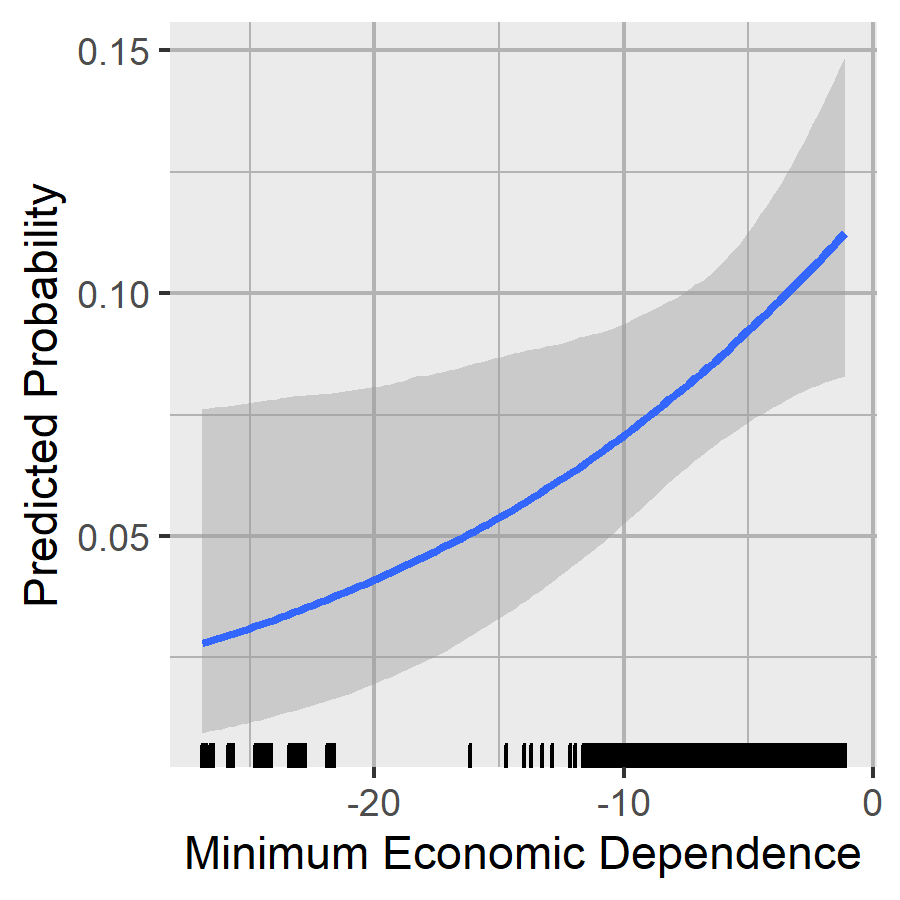
\includegraphics[]{"C:/Users/gwill/Dropbox/Research/Dissertation/Data Analysis/figures/attempts.png"}
\end{figure}

In addition to an increased incentive to negotiate, my theory predicts that states which are highly dependent on each other for their economic wellbeing have greater incentives to reach agreements. Hypothesis \ref{hyp: agreements} posits that this will result in a higher probability that states sign an agreement in a given year. Table \ref{tab: agreements} the results of a model of the probability that states reach an agreement. As before, the mean of the posterior distribution is positive, indicating that higher levels of interdependence are associated with an increase in the probability that states reach an agreement. Ninety-eight percent of the posterior distribution lie above 0, indicating that there is a high degree of certainty regarding the probability of a positive effect. Figure \ref{fig: agreements} displays the marginal effect of economic dependence. The probability of signing an agreement in a given year is roughly four times larger at the high end of the spectrum than the low end.

%%%%% Agreements
\begin{table}[ht]
	\caption{Effect of Economic Interdependence on Probability of Agreements}
	\label{tab: agreements}
	\centering
			\begin{tabular}{rrrr}
			\toprule
			& Mean & SD & Percent Above/Below Zero \\ 
			
			\midrule
			
			Minimum Economic Dependence & 0.06 & 0.02 & 0.02 \\ 
			
			Claim Salience & -0.04 & 0.04 & 0.35 \\ 
			
			River Claim & 0.32 & 0.27 & 0.20 \\ 
			
			Maritime Claim & -0.53 & 0.23 & 0.01 \\ 
			
			Min. Percent Change in GDP & -0.00 & 0.01 & 0.85 \\ 
			
			Government Crisis in Either State & 0.05 & 0.13 & 0.72 \\ 
			
			Civil War in Either State & 0.35 & 0.15 & 0.02 \\ 
			
			Dyadic MID & 0.33 & 0.19 & 0.07 \\ 
			
			Recent MIDs & 0.18 & 0.11 & 0.11 \\ 
			
			Recent Failed CM Attempts & 0.07 & 0.06 & 0.22 \\ 
			
			Recent Successful CM Attempts & 0.62 & 0.08 & 0.00 \\ 
			
			Capability Ratio & -1.73 & 0.63 & 0.01 \\ 
			
			Joint Democracy & 0.29 & 0.16 & 0.06 \\ 
			
			Joint Autocracy & 0.10 & 0.31 & 0.74 \\ 
			
			Defensive Alliance & -0.09 & 0.12 & 0.45 \\ 
			
			Contiguity & 0.28 & 0.21 & 0.18 \\ 
			
			Shared IGO Membership & 0.01 & 0.00 & 0.06 \\ 
			
			Year & -0.03 & 0.01 & 0.01 \\ 
			
			Year$^2$ & 0.44 & 0.18 & 0.02 \\ 
			
			Year$^3$ & -0.00 & 0.00 & 0.07 \\ 
			
			$\alpha_0$ & -0.69 & 0.73 & 0.33 \\ 
			
			$\alpha_{claim}$ & 0.66 & 0.34 &  \\ 
			
			$\alpha_{year}$ & 0.17 & 0.12 &  \\ 
		\bottomrule
		\end{tabular}
\end{table}



\begin{figure}
	\caption{Marginal Effects of Economic Dependence on Agreements. Shaded regions represent 95 percent credible intervals.}
	\label{fig: agreements}
	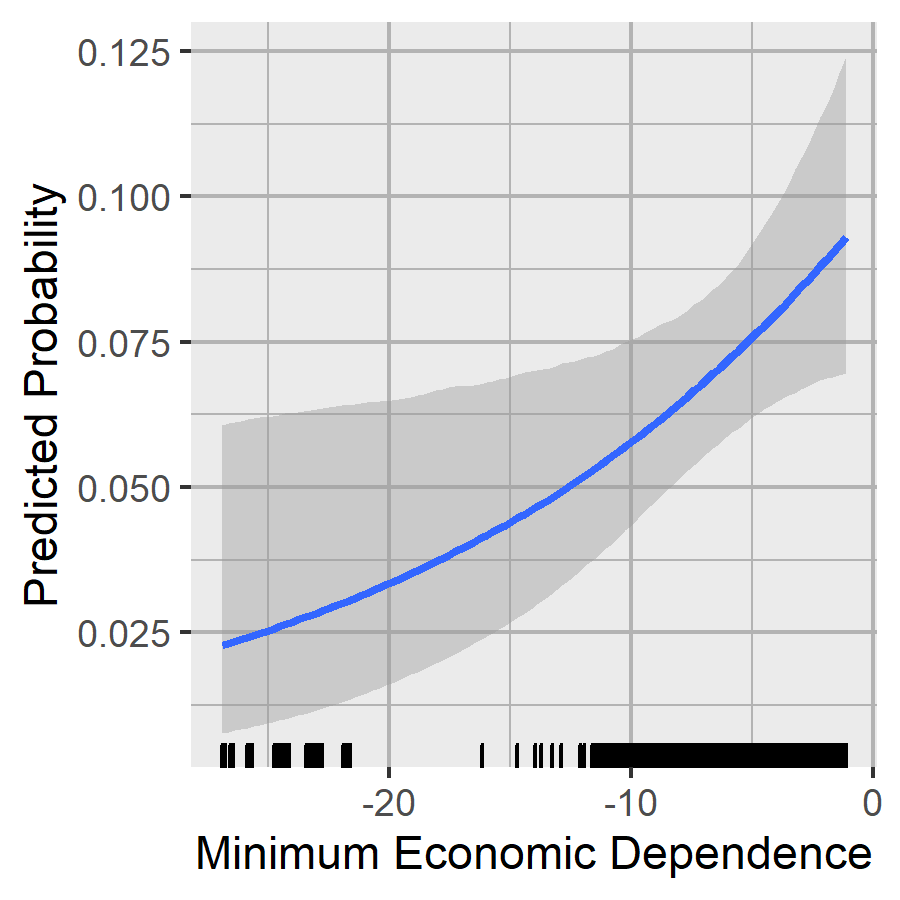
\includegraphics[]{"C:/Users/gwill/Dropbox/Research/Dissertation/Data Analysis/figures/agreements.png"}
\end{figure}

Hypothesis \ref{hyp: concessions} states that highly interdependent states are more likely to sign agreements that involve costly concessions. These results are displayed in Table \ref{tab: concessions}. As before, Ninety-six and eight tenths of the posterior distribution lie above zero, indicating that there is a strong probability that trade dependence has a positive effect. Figure \ref{fig: concessions} displays the marginal effect of economic dependence. As can be seen, the probability of concessions more than doubles from the minimum to the maximum value of economic dependence. However, the substantive effect is lower compared to the other two variables. This is likely due to the fact that, of the three variables, concessions are the most costly.

%%%%% Concessions
\begin{table}[ht]
	\caption{Effect of Economic Interdependence on Probability of Concessions}
	\label{tab: concessions}
	\centering
	\begin{tabular}{rrrr}
		\toprule
		& Mean & SD & Percent Above/Below Zero \\ 
		\midrule
		Minimum Economic Dependence & 0.10 & 0.05 & 3.20 \\ 
		Claim Salience & -0.08 & 0.06 & 20.20 \\ 
		River Claim & 0.22 & 0.43 & 61.90 \\ 
		Maritime Claim & -0.90 & 0.38 & 1.90 \\ 
		Min. Percent Change in GDP & 0.01 & 0.02 & 38.50 \\ 
		Government Crisis in Either State & 0.24 & 0.21 & 25.00 \\ 
		Civil War in Either State & 0.49 & 0.25 & 4.60 \\ 
		Dyadic MID & -0.39 & 0.36 & 27.30 \\ 
		Recent MIDs & 0.18 & 0.21 & 36.90 \\ 
		Recent Failed CM Attempts & -0.06 & 0.09 & 51.60 \\ 
		Recent Successful CM Attempts & 0.78 & 0.12 & 0.00 \\ 
		Capability Ratio & -1.79 & 1.00 & 7.00 \\ 
		Joint Democracy & 0.24 & 0.28 & 38.50 \\ 
		Joint Autocracy & 1.30 & 0.42 & 0.40 \\ 
		Defensive Alliance & -0.14 & 0.21 & 50.60 \\ 
		Contiguity & 0.04 & 0.35 & 92.10 \\
		Shared IGO Membership & 0.01 & 0.01 & 3.40 \\ 
		Year & -0.05 & 0.02 & 1.50 \\ 
		Year$^2$ & 0.65 & 0.34 & 5.90 \\ 
		Year$^3$ & -0.00 & 0.00 & 6.50 \\ 
		$\alpha_0$ & -1.32 & 1.21 & 28.20 \\ 
		$\alpha_{claim}$ & 1.10 & 0.28 &  \\ 
		$\alpha_{year}$ & 0.23 & 0.17 &  \\ 
		\bottomrule
	\end{tabular}
	
\end{table}



\begin{figure}

\caption{Marginal Effects of Economic Dependence on Concessions. Shaded regions represent 95 percent credible intervals.}

\label{fig: concessions}

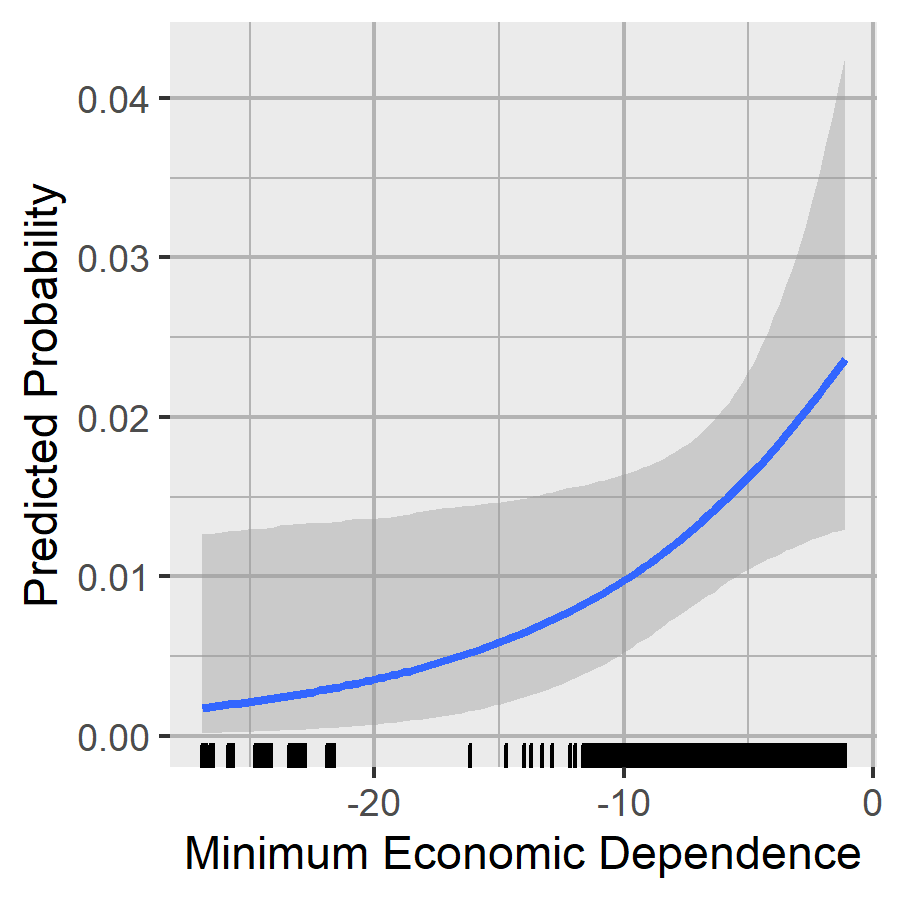
\includegraphics[]{"C:/Users/gwill/Dropbox/Research/Dissertation/Data Analysis/figures/concessions.png"}

\end{figure}

In general, the control variables behave as expected across all three models. Maritime claims less likely to be the subject of peaceful settlement attempts. Ongoing MIDs are associated with a higher level of settlement attempts and agreements but not with more concessions. Recent conflict management attempts are associated with an increased probability of additional all three dependent variables, indicating that attempts tend to cluster together. 

Intriguingly, only one of the control variables that measures domestic support for a state’s leader is strongly associated with the probability of settlement attempts, agreements, or concessions. When one or both states are involved in a civil war within their country, the probability of attempts and agreements increases. This suggests that embattled leaders may have a greater incentive to reach agreements as a means of defraying domestic discontent and/or creating alliances with their opponents. The fact that none of the domestic support controls are associated with a decrease in settlement attempts or agreements may indicate that leaders’ decision-making is primarily based on the potential costs and benefits of resolving the dispute rather than domestic opposition.

In general, the dyadic control variables behave as expected. Higher levels of the capability ratio are associated with a lower probability of agreements and attempts, indicating that high levels of asymmetry in power are associated with less concessions. Joint democracy is associated with a higher probability of attempts and agreements. This effect does not hold for joint autocracy, which may be due to the fact that autocracies are less likely to engage in peaceful conflict management altogether. The number of IGOs which both states belong two is positively associated with attempts and agreements.

\section{Discussion}

The results above support the argument that states which are highly dependent on each other are more likely to pursue and reach peaceful settlements over issue claims. Specifically, leaders are more likely to pursue peaceful settlement attempts, sign agreements, and make concessions over issue claims when domestic businesses have more to lose and more to gain from resolving claims with their opponents. These findings have five implications for scholarly research and policymaking. First, economic interdependence has implications for state behavior beyond reducing armed conflict. Specifically, states may be more likely to use peaceful conflict management strategies to resolve disputes between actors that are highly interdependent. Second, it contributes to the literature on contentious issues by suggesting that the management of these claims is influenced by trade. 

Third, these findings provide additional evidence that the conflict management strategies that states choose are contingent on the extent to which domestic audiences are opposed to settlement. Fourth, policymakers interested in encouraging the settlement of contentious claims may benefit from increasing bilateral economic activity between states. Fifth, it also provides evidence that institutions designed to increase regional integration between states may play a role in promoting regional stability.

The findings in this chapter suggest three avenues for future research. First, researchers may wish to examine whether the effects of economic interdependence are contingent on the salience of claims. It is possible that higher incentives for domestic audiences are more important in the context of highly salient claims which are more likely to face opposition. On the other hand, the effects of economic interdependence may be weaker in the context of highly salient claims due to the fact that it is more difficult for trade to overcome opposition to the settlement. Second, it may be of interest to examine whether the size of the effects of interdependence vary based on issue types. For example, since territorial claims are generally regarded as more salient than other issues, the effects of interdependence may be stronger or weaker over these claims (for the same reasons as overall claim salience). 

Third, future research could examine whether economic interdependence has disparate effects on different types of conflict management. For example previous literature suggests that leaders are more likely to choose arbitration and adjudication when domestic opposition to settlement is high \citep[e.g., ][]{allee2006}. This suggests that states with low levels of interdependence may be more prone to resort to these strategies.

%\section{References}

%\printbibliography[heading=none]

%\end{document}